\documentclass{report}

%subject to pathing issues, remember to change
\input{../../pkgs/preamble}
\input{../../pkgs/macros}
\input{../../pkgs/letterfonts}

\usetikzlibrary{trees}
\title{\Huge{CS212}\\ Lab7 }
\author{\huge{Yan Bogdanovskyy (yawnbo)}}
\date{\today}

\begin{document}

\maketitle
1.\\
\begin{multicols}{2}
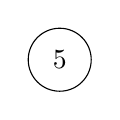
\begin{tikzpicture}[
 every node/.style={circle, draw, minimum size=8mm},
 level distance=15mm,
 level 1/.style={sibling distance=40mm},
 level 2/.style={sibling distance=20mm},
 level 3/.style={sibling distance=10mm},
 level 4/.style={sibling distance=10mm}
]
    \node {5};
\end{tikzpicture}
\\ 2.\\
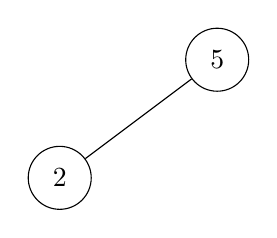
\begin{tikzpicture}[
 every node/.style={circle, draw, minimum size=8mm},
 level distance=15mm,
 level 1/.style={sibling distance=40mm},
 level 2/.style={sibling distance=20mm},
 level 3/.style={sibling distance=10mm},
 level 4/.style={sibling distance=10mm}
]
    \node {5}
        child {node {2}}
				child[missing];
\end{tikzpicture}
\\3.\\
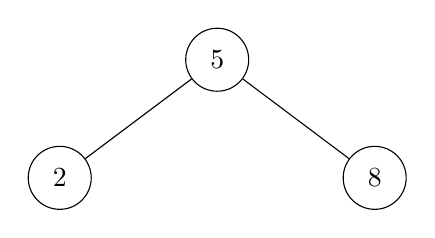
\begin{tikzpicture}[
 every node/.style={circle, draw, minimum size=8mm},
 level distance=15mm,
 level 1/.style={sibling distance=40mm},
 level 2/.style={sibling distance=20mm},
 level 3/.style={sibling distance=10mm},
 level 4/.style={sibling distance=10mm}
]
    \node {5}
        child {node {2}}
        child {node {8}};
\end{tikzpicture}
\\4.\\
\begin{tikzpicture}[
 every node/.style={circle, draw, minimum size=8mm},
 level distance=15mm,
 level 1/.style={sibling distance=40mm},
 level 2/.style={sibling distance=20mm},
 level 3/.style={sibling distance=10mm},
 level 4/.style={sibling distance=10mm}
]
    \node {5}
        child {node {2}
            child {node {1}}
						child[missing]
					}
        child {node {8}};
\end{tikzpicture}
\\5.\\

\begin{tikzpicture}[
 every node/.style={circle, draw, minimum size=8mm},
 level distance=15mm,
 level 1/.style={sibling distance=40mm},
 level 2/.style={sibling distance=20mm},
 level 3/.style={sibling distance=10mm},
 level 4/.style={sibling distance=10mm}
]
\node{5}
    child {node {2}
        child {node{1}
            child {node{0}}
            child[missing]
        }
        child[missing]
    }
    child {node{8}};
\end{tikzpicture}
\\5.1 right rotate node 2\\
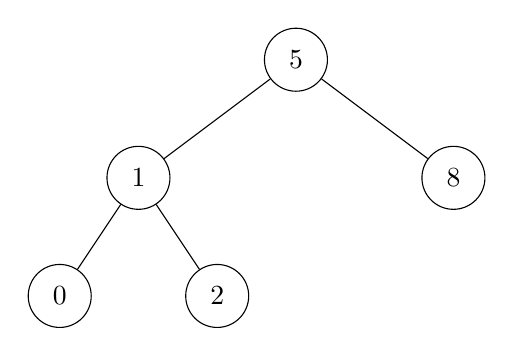
\begin{tikzpicture}[
 every node/.style={circle, draw, minimum size=8mm},
 level distance=15mm,
 level 1/.style={sibling distance=40mm},
 level 2/.style={sibling distance=20mm},
 level 3/.style={sibling distance=10mm},
 level 4/.style={sibling distance=10mm}
]
\node{5}
	child{node {1}
		child{node{0}}
		child{node{2}}
	}
	child{node{8}};
\end{tikzpicture}

\\6.\\
\begin{tikzpicture}[
 every node/.style={circle, draw, minimum size=8mm},
 level distance=15mm,
 level 1/.style={sibling distance=40mm},
 level 2/.style={sibling distance=20mm},
 level 3/.style={sibling distance=10mm},
 level 4/.style={sibling distance=10mm}
]

\node{5}
	child{node {1}
		child{node{0}}
		child{node{2}
			child[missing]
			child{node{3}}
		}
	}
	child{node{8}};
\end{tikzpicture}
\\6.1 need a left-right rebalance at root because our bf is -2 and first subtree node is bf $ > $ 0.\\
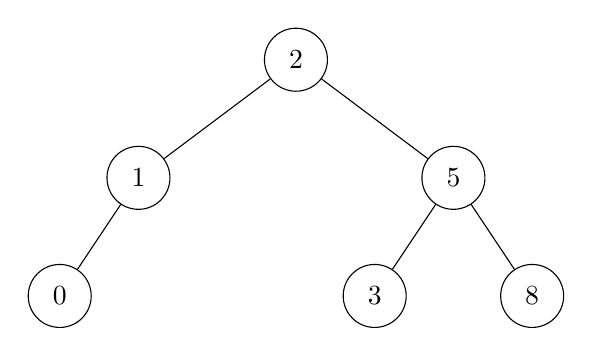
\begin{tikzpicture}[
 every node/.style={circle, draw, minimum size=8mm},
 level distance=15mm,
 level 1/.style={sibling distance=40mm},
 level 2/.style={sibling distance=20mm},
 level 3/.style={sibling distance=10mm},
 level 4/.style={sibling distance=10mm}
]

\node{2}
	child{node {1}
		child{node{0}}
		child[missing]
	}
	child{node{5}
		child{node{3}}
	child{node{8}}
};
\end{tikzpicture}
\\7.\\

\begin{tikzpicture}[
 every node/.style={circle, draw, minimum size=8mm},
 level distance=15mm,
 level 1/.style={sibling distance=40mm},
 level 2/.style={sibling distance=20mm},
 level 3/.style={sibling distance=10mm},
 level 4/.style={sibling distance=10mm}
]

\node{2}
	child{node {1}
		child{node{0}}
		child[missing]
	}
	child{node{5}
		child{node{3}
			child[missing]
			child{node{4}}
		}
	child{node{8}}
};
\end{tikzpicture}
\\8.\\
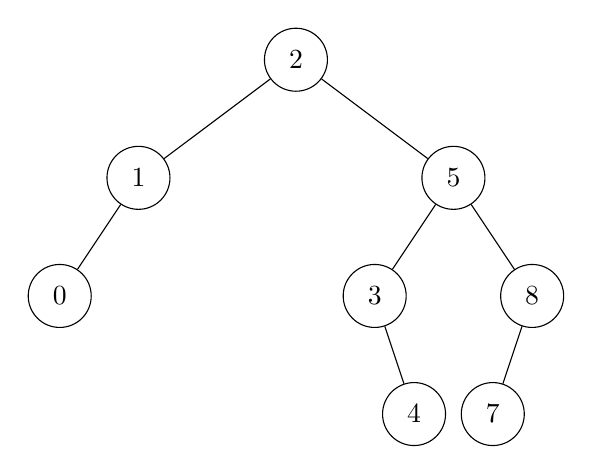
\begin{tikzpicture}[
 every node/.style={circle, draw, minimum size=8mm},
 level distance=15mm,
 level 1/.style={sibling distance=40mm},
 level 2/.style={sibling distance=20mm},
 level 3/.style={sibling distance=10mm},
 level 4/.style={sibling distance=10mm}
]

\node{2}
	child{node {1}
		child{node{0}}
		child[missing]
	}
	child{node{5}
		child{node{3}
			child[missing]
			child{node{4}}
		}
	child{node{8}
		child{node{7}}
		child[missing]
	}
};
\end{tikzpicture}
\newpage
\\9. i give up on drawing inbetween steps. 6 becomes child of 7 making for a -2 height at node 8 and requiring a right rotation\\
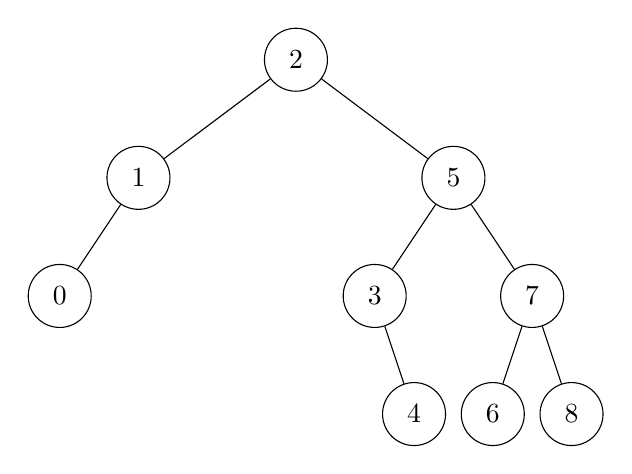
\begin{tikzpicture}[
 every node/.style={circle, draw, minimum size=8mm},
 level distance=15mm,
 level 1/.style={sibling distance=40mm},
 level 2/.style={sibling distance=20mm},
 level 3/.style={sibling distance=10mm},
 level 4/.style={sibling distance=10mm}
]

\node{2}
	child{node {1}
		child{node{0}}
		child[missing]
	}
	child{node{5}
		child{node{3}
			child[missing]
			child{node{4}}
		}
		child{node{7}
			child{node{6}}
			child{node{8}}
		}
};
\end{tikzpicture}
\\10. inserting a 9 will cause the root node to have a bf of (-2 + 4) = 2 which requires a rebalancing of rightright or a simple left rotation\\

\begin{tikzpicture}[
 every node/.style={circle, draw, minimum size=8mm},
 level distance=15mm,
 level 1/.style={sibling distance=40mm},
 level 2/.style={sibling distance=20mm},
 level 3/.style={sibling distance=10mm},
 level 4/.style={sibling distance=10mm}
]

\node{5}
	child{node {2}
		child{node{1}
			child{node{0}}
			child[missing]
		}
		child{node{3}
			child[missing]
			child{node{4}}
		}
	}
	child{node{7}
		child{node{6}}
		child{node{8}
			child[missing]
			child{node{9}}
		}
	};
};
\end{tikzpicture}
\\11. Finally, inserting a 10 will cause a bf of 2 at node 8 which is a right right violation needing just a left rotation at 8.\\
\begin{tikzpicture}[
 every node/.style={circle, draw, minimum size=8mm},
 level distance=15mm,
 level 1/.style={sibling distance=40mm},
 level 2/.style={sibling distance=20mm},
 level 3/.style={sibling distance=10mm},
 level 4/.style={sibling distance=10mm}
]

\node{5}
	child{node {2}
		child{node{1}
			child{node{0}}
			child[missing]
		}
		child{node{3}
			child[missing]
			child{node{4}}
		}
	}
	child{node{7}
		child{node{6}}
		child{node{9}
			child{node{8}}
			child{node{10}}
		}
	};
};
\end{tikzpicture}
\paragraph{\\ \\Part 2 value removal.\\}
\\1. remove root and set equal to rightmost value in left subtree\\
\begin{tikzpicture}[
 every node/.style={circle, draw, minimum size=8mm},
 level distance=15mm,
 level 1/.style={sibling distance=40mm},
 level 2/.style={sibling distance=20mm},
 level 3/.style={sibling distance=10mm},
 level 4/.style={sibling distance=10mm}
]

\node{4}
	child{node {2}
		child{node{1}
			child{node{0}}
			child[missing]
		}
		child{node{3}}
	}
	child{node{7}
		child{node{6}}
		child{node{9}
			child{node{8}}
			child{node{10}}
		}
	};
};
\end{tikzpicture}
\\2.\\

\begin{tikzpicture}[
 every node/.style={circle, draw, minimum size=8mm},
 level distance=15mm,
 level 1/.style={sibling distance=40mm},
 level 2/.style={sibling distance=20mm},
 level 3/.style={sibling distance=10mm},
 level 4/.style={sibling distance=10mm}
]

\node{4}
	child{node {2}
		child{node{1}
			child{node{0}}
			child[missing]
		}
		child{node{3}}
	}
	child{node{7}
		child{node{6}}
		child{node{9}
			child{node{8}}
			child[missing]
		}
	};
};
\end{tikzpicture}
\\3. sub root of left subtree with first node on the left\\
\begin{tikzpicture}[
 every node/.style={circle, draw, minimum size=8mm},
 level distance=15mm,
 level 1/.style={sibling distance=40mm},
 level 2/.style={sibling distance=20mm},
 level 3/.style={sibling distance=10mm},
 level 4/.style={sibling distance=10mm}
]

\node{4}
	child{node {1}
			child{node{0}}
			child{node{3}}
	}
	child{node{7}
		child{node{6}}
		child{node{9}
			child{node{8}}
			child[missing]
		}
	};
};
\end{tikzpicture}
\\4.\\
\begin{tikzpicture}[
 every node/.style={circle, draw, minimum size=8mm},
 level distance=15mm,
 level 1/.style={sibling distance=40mm},
 level 2/.style={sibling distance=20mm},
 level 3/.style={sibling distance=10mm},
 level 4/.style={sibling distance=10mm}
]

\node{4}
	child{node {1}
			child{node{0}}
			child{node{3}}
	}
	child{node{7}
		child{node{6}}
		child{node{9}}
	};
};
\end{tikzpicture}
\paragraph{I give up on writing it like this here's the rest\\}
\includegraphics[angle=-90, width=\textwidth]{avl_tree.png}
\end{multicols}
\end{document}
